\documentclass[10pt]{book}
\usepackage{ifthen}

\newboolean{in_color}
\newboolean{sevenbytenbooksize}
\newboolean{ipadsize}   % for the ipad, Duh.

\setboolean{in_color}{true}
%\setboolean{booksize}{false}
\setboolean{sevenbytenbooksize}{true}
\setboolean{ipadsize}{false}


\usepackage{amsmath}
\usepackage{amssymb}
\usepackage{amsthm}

%
%	Note how the iPad version differs from the booksize only in 
% the size of the margins.
%
% 
%
					%% Layout for printed book through Amazon CreateSpace, perfect bound,
					%% 7x10 ``journal'' size

\ifthenelse{\boolean{ipadsize}}{\usepackage[paperheight=620pt,paperwidth=395pt, textheight=550pt,
textwidth=345pt, includeheadfoot, hcentering=true]{geometry}}{}


\ifthenelse{\boolean{sevenbytenbooksize}}{\usepackage[paperheight=10in,paperwidth=7in, textheight=550pt,
textwidth=345pt, inner=1in,includeheadfoot]{geometry}}{}



\usepackage{layout}
\usepackage{graphicx}
\usepackage{multicol}
\usepackage{tikz}
\usetikzlibrary{calc}
\usepackage{makeidx}

\usepackage{changepage}
\usepackage{ulem}
\usepackage{xcolor}
\usepackage[bookmarksnumbered,linkbordercolor=white]{hyperref}

\usepackage{fancyhdr}
\usepackage{calc}

\pagestyle{fancy}
\fancyhead{}
\fancyfoot{}
\renewcommand{\chaptermark}[1]{\markboth{\chaptername\ \thechapter\ \ \ \ {#1}}{}}
\renewcommand{\sectionmark}[1]{\markright{\thesection\ \ \ \  #1}}
\fancyhf{}         %Clears all header and footer fields, in preparation.
%\fancyheadoffset[LE,RO]{\marginparsep}
%\addtolength{\headwidth}{\marginparwidth}

%\ifthenelse{\boolean{sevenbytenbooksize}}{\fancyhfoffset[LE,RO]{30pt}}{}  
		%  CreateSpace text size but really not needed as its an ``else''
		%  from above
		
\fancyhfoffset[LE,RO]{30pt}
\fancyfoot[LE,RO]{\textbf{\thepage}} %Displays the page number in bold in the header,
                       % to the left on even pages and to the right on odd pages.
                                     
\fancyhead[LE]{\nouppercase{\leftmark}}
      %Displays the upper-level (chapter) information---
      % as determined above---in non-upper case in the header, 
      %to the right on even pages.
\fancyhead[RO]{\rightmark}
			%Displays the lower-level (section) information---as
      % determined above---in the header, to the left on odd pages.
\renewcommand{\headrulewidth}{0pt}
\renewcommand{\footrulewidth}{0pt}
	%Underlines the header and footer. (Set to 0pt if not required).

\makeatletter
\def\@makechapterhead#1{%
  {\parindent \z@ \raggedright \reset@font
    \large
    \resizebox{1.6cm}{2cm}{\thechapter}\ \ %
		\if \thechapter 1
%
\begin{tikzpicture}
%Chapter 1 Pic 1
\begin{scope}
\draw (-1,0)--(2,0);
\draw (0,-.5)--(0,3);
\draw [thick] (-.5,-.5)--(1.5,1.5);
\draw [thick] (-.5,2.5)--(1.5,.5);
\draw  (-1.1,-.6)--(2.1,-.6)--(2.1,3.1)--(-1.1,3.1)--cycle;
\end{scope}

%Chapter 1 pic 2
\begin{scope}[shift={(3.4,0)}]
\draw (-1,0)--(2,0);
\draw (0,-.5)--(0,3);
\draw [thick] (-.5,1.5)--(1.5,-.5);
\draw [thick] (-.5,2.5)--(1.5,.5);
\draw  (-1.1,-.6)--(2.1,-.6)--(2.1,3.1)--(-1.1,3.1)--cycle;
\end{scope}

%Chapter 1 pic 3
\begin{scope}[shift={(6.8,0)}]
\draw (-1,0)--(2,0);
\draw (0,-.5)--(0,3);
\draw [very thick] (-.5,1.5)--(1.5,-.5);
%\draw [thick] (-.5,2.5)--(1.5,.5);
\draw (-1.1,-.6)--(2.1,-.6)--(2.1,3.1)--(-1.1,3.1)--cycle;
\end{scope}
\end{tikzpicture}
%
\else \if \thechapter 2
%
\begin{tikzpicture}[>=latex]

%chapter 2 pic 1
\begin{scope}
\draw (-1,0)--(2,0);
\draw (0,-.5)--(0,3);
\draw [thick,->] (0,0)--(-.5,1.5);
\draw [thick,->] (0,0)--(1.5,.75);
\draw [thick,->,dashed,gray] (-.5,1.5)--(1,2.25);
\draw [thick,->,dashed,gray] (1.5,.75)--(1,2.25);
\draw [thick,->] (0,0)--(1,2.25);
\draw  (-1.1,-.6)--(2.1,-.6)--(2.1,3.1)--(-1.1,3.1)--cycle;
\end{scope}

%Chapter 2 pic 2
\begin{scope}[shift={(3.4,0)}]
\draw (-1,0) -- (2,0);
\draw (0,-.5)--(0,3);
\draw [thick] (0,1) circle (.5cm);
\draw [thick, gray, rotate around={45:(1.1,1)}] (1.1,1) ellipse (.6cm and .4cm);
%\draw [thick,gray] (.6,1) node [right] {$A'$} .. (.6,.5) .. (1.65,1) .. (1.65,1.5) node [below left] {$B'$} ..cycle;
%\node [above] at (.817cm,1.28cm) {$A$};
%\fill (.817cm,1.28cm) circle (.04cm); 
\fill [rotate around={45:(1.1,1)}](.5,1) circle (.04cm) node [above right] {$A'$};
\fill [rotate around={45:(1.1,1)}](1.1,1.4) circle (.04cm) node [above ] {$B'$};

\fill (0,1.5) circle (.04) node [above right] {$B$}; 
\fill (-.5,1) circle (.04) node [right] {$A$};

\draw  (-1.1,-.6)--(2.1,-.6)--(2.1,3.1)--(-1.1,3.1)--cycle;
\end{scope}

%chapter 2 pic 3
\begin{scope}[shift={(6.8,0)}]
\draw (-1,0)--(2,0);
\draw (0,-.5)--(0,3);

\draw (-1,-.5)--(1.8,.9);
\draw [->,thick] (0,0)--(1,.5);
\draw [->,thick,dashed] (0,0)--(-.5,1.5);
\draw (-1,1.25)--(1.8,2.65);
\draw [->,thick] (-.5,1.5)--(.5,2);

\draw  (-1.1,-.6)--(2.1,-.6)--(2.1,3.1)--(-1.1,3.1)--cycle;\end{scope}
\end{tikzpicture}
%
\else \if \thechapter 3
%
\begin{tikzpicture}[>=latex]

%chapter 3 pic 1
\begin{scope}
\draw (-1,0)--(2,0);
\draw (0,-.5)--(0,3);
\draw  (-1.1,-.6)--(2.1,-.6)--(2.1,3.1)--(-1.1,3.1)--cycle;

\draw [->,thick] (0,0)--(-.5,1.5);
\draw [->,thick] (0,0)--(1,.5);
\draw [->,thick,dashed,gray] (-.5,1.5)--(.5,2);
\draw [->,thick,dashed,gray] (1,.5)--(.5,2);

\end{scope}

%chapter 3 pic 2
\begin{scope}[shift={(3.4,0)}]
\draw (-1,0) -- (2,0);
\draw (0,-.5)--(0,3);
\draw  (-1.1,-.6)--(2.1,-.6)--(2.1,3.1)--(-1.1,3.1)--cycle;

\draw [->,thick] (0,0)--(-.5,1);
\draw [->,thick] (0,0)--(1.5,.5);
\draw [->,thick,dashed,gray] (-.5,1)--(1,1.5);
\draw [->,thick,dashed,gray] (1.5,.5)--(1,1.5);

\end{scope}

%chapter 3 pic 3
\begin{scope}[shift={(6.8,0)}]
\draw (-1,0)--(2,0);
\draw (0,-.5)--(0,3);
\draw  (-1.1,-.6)--(2.1,-.6)--(2.1,3.1)--(-1.1,3.1)--cycle;

\draw [->,thick] (0,0)--(1.25,-.25);
\draw [->,thick] (0,0)--(-.25,2.25);
\draw [->,thick,dashed,gray] (1.25,-.25)--(1,2);
\draw [->,thick,dashed,gray] (-.25,2.25)--(1,2);
\end{scope}

\end{tikzpicture}
%
\else \if \thechapter 4
%
\begin{tikzpicture}[>=latex]

%chapter 4 pic 1
\begin{scope}
\draw (-1,0)--(2,0);
\draw (0,-.5)--(0,3);
\draw  (-1.1,-.6)--(2.1,-.6)--(2.1,3.1)--(-1.1,3.1)--cycle;

\draw [->,thick] (0,0)--(1,.5);
\draw [->,thick] (0,0)--(.5,1);
\draw [->,thick,dashed,gray] (1,.5)--(1.5,1.5);
\draw [->,thick,dashed,gray] (.5,1)--(1.5,1.5);

\end{scope}

%chapter 4 pic 2
\begin{scope}[shift={(3.4,0)}]
\draw (-1,0) -- (2,0);
\draw (0,-.5)--(0,3);
\draw  (-1.1,-.6)--(2.1,-.6)--(2.1,3.1)--(-1.1,3.1)--cycle;

\draw [->,thick] (0,0)--(-1,1);
\draw [->,thick] (0,0)--(1,1);
\draw (0,.5) circle (.5);
\fill (0,0) circle (.04); 
\fill (-.5,.5) circle (.04); 
\fill (.5,.5) circle (.04); 
\fill (0,1) circle (.04); 

\end{scope}

%chapter 4 pic 3
\begin{scope}[shift={(6.8,0)}]
\draw (-1,0)--(2,0);
\draw (0,-.5)--(0,3);
\draw  (-1.1,-.6)--(2.1,-.6)--(2.1,3.1)--(-1.1,3.1)--cycle;

\draw [->,thick] (0,0)--(-.5,.5);
\draw [->,thick] (0,0)--(1.5,1.5);
\fill (0,0) circle (.04); 
\fill (-.25,.25) circle (.04); 
\fill (.75,.75) circle (.04); 
\fill (.5,1) circle (.04); 
%\draw (.25,.5) circle (.55);

\draw [rotate around={45:(.25,.5)}] (.25,.5) ellipse (.57 and .5);

\end{scope}

\end{tikzpicture}
%
\else \if \thechapter 5
%
\begin{tikzpicture}[>=latex]

%chapter 5 pic 1
\begin{scope}
\draw (-1,0)--(2,0);
\draw (0,-.5)--(0,3);

\draw (-1,-.5)--(1.8,.9);
\draw [->,thick] (0,0)--(1,.5);
\draw [->,thick,dashed] (0,0)--(-.5,1.5);
\draw (-1,1.25)--(1.8,2.65);
\draw [->,thick] (-.5,1.5)--(.5,2);

\draw  (-1.1,-.6)--(2.1,-.6)--(2.1,3.1)--(-1.1,3.1)--cycle;
\end{scope}

%chapter 5 pic 2
\begin{scope}[shift={(3.4,0)}]
\draw (-1,0)--(2,0);
\draw (0,-.5)--(0,3);
\draw  (-1.1,-.6)--(2.1,-.6)--(2.1,3.1)--(-1.1,3.1)--cycle;

\draw [->,thick] (0,0)--(1.25,-.25);
\draw [->,thick] (0,0)--(-.25,2.25);
\draw [->,thick,dashed,gray] (1.25,-.25)--(1,2);
\draw [->,thick,dashed,gray] (-.25,2.25)--(1,2);
\end{scope}

%chapter 5 pic 3
\begin{scope}[shift={(6.8,0)}]
\draw (-1,0)--(2,0);
\draw (0,-.5)--(0,3);
\draw  (-1.1,-.6)--(2.1,-.6)--(2.1,3.1)--(-1.1,3.1)--cycle;

\draw [->,thick] (0,0)--(-.5,.5);
\draw [->,thick] (0,0)--(1.5,1.5);
\fill (0,0) circle (.04); 
\fill (-.25,.25) circle (.04); 
\fill (.75,.75) circle (.04); 
\fill (.5,1) circle (.04); 
%\draw (.25,.5) circle (.55);

\draw [rotate around={45:(.25,.5)}] (.25,.5) ellipse (.57 and .5);

\end{scope}

\end{tikzpicture}
%
\else \if \thechapter A
%
\begin{tikzpicture}[>=latex]

%appendix pic 1 = chapter 2 pic 3
\begin{scope}
\draw (-1,0)--(2,0);
\draw (0,-.5)--(0,3);

\draw (-1,-.5)--(1.8,.9);
\draw [->,thick] (0,0)--(1,.5);
\draw [->,thick,dashed] (0,0)--(-.5,1.5);
\draw (-1,1.25)--(1.8,2.65);
\draw [->,thick] (-.5,1.5)--(.5,2);

\draw  (-1.1,-.6)--(2.1,-.6)--(2.1,3.1)--(-1.1,3.1)--cycle;
\end{scope}

%appendix pic 2 = chapter 3 pic 3
\begin{scope}[shift={(3.4,0)}]
\draw (-1,0)--(2,0);
\draw (0,-.5)--(0,3);
\draw  (-1.1,-.6)--(2.1,-.6)--(2.1,3.1)--(-1.1,3.1)--cycle;

\draw [->,thick] (0,0)--(1.25,-.25);
\draw [->,thick] (0,0)--(-.25,2.25);
\draw [->,thick,dashed,gray] (1.25,-.25)--(1,2);
\draw [->,thick,dashed,gray] (-.25,2.25)--(1,2);
\end{scope}

%appendix pic 3 = chapter 4 pic 3
\begin{scope}[shift={(6.8,0)}]
\draw (-1,0)--(2,0);
\draw (0,-.5)--(0,3);
\draw  (-1.1,-.6)--(2.1,-.6)--(2.1,3.1)--(-1.1,3.1)--cycle;

\draw [->,thick] (0,0)--(-.5,.5);
\draw [->,thick] (0,0)--(1.5,1.5);
\fill (0,0) circle (.04); 
\fill (-.25,.25) circle (.04); 
\fill (.75,.75) circle (.04); 
\fill (.5,1) circle (.04); 
%\draw (.25,.5) circle (.55);

\draw [rotate around={45:(.25,.5)}] (.25,.5) ellipse (.57 and .5);

\end{scope}

\end{tikzpicture}

\fi
\fi
\fi
\fi
\fi
\fi


    \reset@font\LARGE\scshape\bfseries\strut \textsc #1
    \par\vskip 10\p@
    \hrule height 1pt
    \vskip 50\p@
  }}
  
%\makeatletter
\def\@makesectionhead#1{%
	 {\reset@font\LARGE\itshape\bfseries\strut #1 \thechapter.\thesection \ #1
	 }}


\makeindex

\normalsize 


\newcommand{\noin}{\noindent}
\newcommand{\ds}{\displaystyle}
\newcommand{\vs}[1]{\vskip #1in}
\newcommand{\tbf}[1]{\textbf{#1}}
\newcommand{\dds}{\displaystyle}
\newcommand{\bmx}[1]{\left[\hskip -3pt\begin{array}{#1} }
\newcommand{\emx}{\end{array}\hskip -3pt\right]}
\newcommand{\bdt}[1]{\left| \begin{array}{#1} }
\newcommand{\edt}{\end{array} \right|}

\newcommand{\btz}{\begin{center}\begin{tikzpicture}}
\newcommand{\etz}{\end{tikzpicture}\end{center}}

\newcommand{\vx}[1][]{\ensuremath{\vec{x_{#1}}}}
\newcommand{\vxp}{\ensuremath{\vec{x_p}}}
\newcommand{\vu}{\ensuremath{\vec{u}}}
\newcommand{\vv}{\ensuremath{\vec{v}}}
\newcommand{\vy}{\ensuremath{\vec{y}}}
\newcommand{\vz}{\ensuremath{\vec{z}}}
\newcommand{\vb}{\ensuremath{\vec{b}}}
\newcommand{\vw}{\ensuremath{\vec{w}}}
\newcommand{\veone}{\ensuremath{\vec{e_1}}}
\newcommand{\vetwo}{\ensuremath{\vec{e_2}}}
\newcommand{\vethree}{\ensuremath{\vec{e_3}}}
\newcommand{\vei}{\ensuremath{\vec{e_i}}}
\newcommand{\ven}[1]{\ensuremath{\vec{e_{#1}}}}
\newcommand{\rr}[1]{\ensuremath{\mathbb{R}^{#1}}}
\newcommand{\zero}{\ensuremath{\vec{\text{\it 0}}}}
\newcommand{\vect}[1]{\ensuremath{\vec{#1}}}
\newcommand{\arref}{\ensuremath{\overrightarrow{\text{rref}}}}
\newcommand{\vectt}[2]{\ensuremath{\bmx{c}#1\\#2\emx}}
\newcommand{\vecttt}[3]{\ensuremath{\bmx{c}#1\\#2\\#3\emx}}

\newcommand{\ttmm}{$M$}
\newcommand{\mm}{\texttt{M}}
\newcommand{\ii}[1]{\ensuremath{I_{#1}}}
\newcommand{\tta}{\ensuremath{A}}
\newcommand{\ttb}{\ensuremath{B}}
\newcommand{\ttc}{\ensuremath{C}}
\newcommand{\ttd}{\ensuremath{D}}
\newcommand{\ttm}{\ensuremath{M}}
\newcommand{\ttx}{\ensuremath{X}}
\newcommand{\tti}{\ensuremath{I}}
\newcommand{\tty}{\ensuremath{Y}}
\newcommand{\ttp}{\ensuremath{P}}
\newcommand{\ttat}{\ensuremath{A^T}}
\newcommand{\ttbt}{\ensuremath{B^T}}
\newcommand{\ttct}{\ensuremath{C^T}}
\newcommand{\ttdt}{\ensuremath{D^T}}
\newcommand{\ttmt}{\ensuremath{M^T}}
\newcommand{\ttxt}{\ensuremath{X^T}}
\newcommand{\ttit}{\ensuremath{I^T}}
\newcommand{\ttyt}{\ensuremath{Y^T}}
\newcommand{\ttai}{\ensuremath{A^{-1}}}
\newcommand{\ttbi}{\ensuremath{B^{-1}}}
\newcommand{\ttxi}{\ensuremath{X^{-1}}}
\newcommand{\ttpi}{\ensuremath{P^{-1}}}
\newcommand{\ttaxb}{\ensuremath{\tta\vx=\vb}}
\newcommand{\ttaxo}{\ensuremath{\tta\vx=\zero}}
\newcommand{\eyetwo}{\ensuremath{\bmx{cc}1&0\\0&1\emx}}
\newcommand{\eyethree}{\ensuremath{\bmx{ccc}1&0&0\\0&1&0\\0&0&1\emx}}
\newcommand{\eyefour}{\ensuremath{\bmx{cccc}1&0&0&0\\0&1&0&0\\0&0&1&0\\0&0&0&1\emx}}
\newcommand{\ma}{\ensuremath{A}}
\newcommand{\mb}{\ensuremath{B}}
\newcommand{\mc}{\ensuremath{C}}
\newcommand{\md}{\ensuremath{D}}
\newcommand{\tto}{\textbf{0}}
\renewcommand{\det}[1]{\text{det}\ensuremath{\left(#1\right)}}
\newcommand{\tr}{$^\text{\tt T}$}
\newcommand{\lda}{\ensuremath{\lambda}}
\newcommand{\rref}{reduced row echelon form}
\newcommand{\Rref}{Reduced row echelon form}
\newcommand{\el}{eigenvalue}
\newcommand{\ev}{eigenvector}
\newcommand{\realn}{\ensuremath{\mathbb{R}^n}}
\newcommand{\realm}{\ensuremath{\mathbb{R}^m}}
\newcommand{\realnm}{\ensuremath{\mathbb{R}^n\rightarrow\mathbb{R}^m}}
\newcommand{\real}[1]{\ensuremath{\mathbb{R}^{#1}}}
\newcommand{\rrr}[2]{\ensuremath{\mathbb{R}^{#1}\rightarrow\mathbb{R}^{#2}}}
\newcommand{\TT}{\ensuremath{[\, T\, ]}}


%  Some TiKZ  shortcuts to help make drawing 3D vectors faster.
%
\newcommand{\drawvect}[7]{\draw [#4] (0,0,0) -- (#1,0,0) -- (#1,#2,0) -- (#1,#2,#3);
  \draw [#5] (0,0,0) -- (#1,#2,#3) node [#6] {#7};}
\newcommand{\drawjustvect}[7]{\draw [#5] (0,0,0) -- (#1,#2,#3) node [#6] {#7};}

\newcommand{\drawxaxis}[4]{\draw [->] (#1,0,0) -- (#2,0,0) node [below left] {$x$};
\foreach \x in {#3,...,#4}
 {\draw (\x,-.1,0)--(\x,.1,0); } }
\newcommand{\drawyaxis}[4]{\draw [->] (0,#1,0) -- (0,#2,0) node [right] {$y$};
\foreach \y in {#3,...,#4}
 {\draw (0,\y,-.1)--(0,\y,.1); }; }
\newcommand{\drawzaxis}[4]{\draw [->] (0,0,#1) -- (0,0,#2) node [above] {$z$};
\foreach \z in {#3,...,#4}
 {\draw (0,-.1,\z)--(0,.1,\z); }; }
%
% 
% Draws the VMI Spider in TikZ
%
\newcommand{\vmispider}[1][]
{\begin{scope}[#1]
	\draw  (-2,2) -- (0,-1) -- (2,2);
	\draw  (-1,-1) -- (-1,2) -- (0,1) -- (1,2) -- (1,-1);
	\draw  (-1,2.5) -- (1,2.5);
	\draw  (-1,-1.5) -- (1,-1.5);
	\draw  (0,-1.5) -- (0,2.5);
\end{scope}
}
%
% Draws the unit square, easy to transform
%
\newcommand{\unitsquare}[1][]
{\begin{scope}
	\draw [#1] (0,0) node (A) {} -- (1,0) node (B) {} -- (1,1) node (C) {} -- (0,1) node (D) {} -- cycle;
	\draw [->,>=latex,#1,ultra thin] (0,.25)--(1,.25);
	\draw [->,>=latex,#1,ultra thin] (0,.5)--(1,.5);
	\draw [->,>=latex,#1,ultra thin] (0,.75)--(1,.75);
	\filldraw [black]  (A) circle (2pt);%black
	\filldraw [fill=white,thick]  (B) ++(-2pt,-2pt) rectangle ++(4pt,4pt);%red
	\filldraw [fill=white,thick]  (C) circle (2pt);%blue
	\filldraw [fill=white,thick]  (D) ++(-2.5pt,-2.5pt) -- ++(5pt,0pt) -- ++(-2.5pt,5pt) -- cycle;%green
	\end{scope}
}
%
% Draws unit square for cover image
%
\newcommand{\unitsquarecover}[1][]
{\begin{scope}
	\draw [#1] (0,0) node (A) {} -- (1,0) node (B) {} -- (1,1) node (C) {} -- (0,1) node (D) {} -- cycle;
	\draw [->,>=latex,#1,thin] (0,.25)--(1,.25);
	\draw [->,>=latex,#1, thin] (0,.5)--(1,.5);
	\draw [->,>=latex,#1, thin] (0,.75)--(1,.75);
	\filldraw [black]  (A) circle (2pt);%black
	\draw [#1,ultra thick]  (B) ++(-2pt,-2pt) rectangle ++(4pt,4pt);%red
	\draw [ultra thick]  (C) circle (2pt);%blue
	\draw [#1,ultra thick]  (D) ++(-2.5pt,-2.5pt) -- ++(5pt,0pt) -- ++(-2.5pt,5pt) -- cycle;%green
	\end{scope}
}
%
% Draws unit square without the arrows in the middle.
%
\newcommand{\unitsquarewithoutarrows}[1][]
{\begin{scope}
	\draw [#1] (0,0) node (A) {} -- (1,0) node (B) {} -- (1,1) node (C) {} -- (0,1) node (D) {} -- cycle;
	\filldraw [black]  (A) circle (2pt);%black
	\filldraw [fill=white,thick]  (B) ++(-2pt,-2pt) rectangle ++(4pt,4pt);%red
	\filldraw [fill=white,thick]  (C) circle (2pt);%blue
	\filldraw [fill=white,thick]  (D) ++(-2.5pt,-2.5pt) -- ++(5pt,0pt) -- ++(-2.5pt,5pt) -- cycle;%green
	\end{scope}
}

%
% Draw x and y tick marks
%
\newcommand{\drawxticks}[1]
{\foreach \x in {#1}
		{\draw  (\x,-.1)--(\x,.1);
			};
}
\newcommand{\drawyticks}[1]
{\foreach \x in {#1}
		{\draw  (-.1,\x)--(.1,\x);
			};
}

\newcommand{\drawxlines}[3]
{\draw[<->] (#1,0) -- (#2,0) node [right] {$x$};
\foreach \x in {#3}
		{\draw  (\x,-.1)--(\x,.1);
			};
}

\newcommand{\drawylines}[3]
{\draw[<->] (0,#1) -- (0,#2) node [above] {$y$};
\foreach \x in {#3}
		{\draw  (-.1,\x)--(.1,\x);
			};
}

%\ifthenelse{\boolean{booksize}}{% Begin if booksize
%\newcommand{\settikzpagecorners}{\begin{tikzpicture}[remember picture, overlay]
%\node [xshift=1in+\oddsidemargin-10pt,yshift=\paperheight-1in-\topmargin-\headheight-\headsep-\textheight-\footskip] (oddpagebottom) at (current page.south west)  {};
%\node [xshift=1in+\evensidemargin-10pt,yshift=\paperheight-1in-\topmargin-\headheight-\headsep-\textheight-\footskip] (evenpagebottom) at (current page.south west) {};
%\node [xshift=1in+\oddsidemargin-10pt,yshift=-1in-\topmargin-\headheight-\headsep] (oddpagetop) at (current page.north west)  {};
%\node [xshift=1in+\evensidemargin-10pt,yshift=-1in-\topmargin-\headheight-\headsep] (evenpagetop) at (current page.north west) {};
%\end{tikzpicture}
%}
%}%  Ends if booksize
%{%  Begins Else not booksize
%\ifthenelse{\boolean{amazonsize}}{% Begin if amazonsize
%\newcommand{\settikzpagecorners}{\begin{tikzpicture}[remember picture, overlay]
%\ifthenelse{\boolean{ipad}}
%{\node [xshift=1in+\oddsidemargin-10pt,yshift=\paperheight-.5in-\textheight-\footskip+15pt] (oddpagebottom) at (current page.south west)  {};
%\node [xshift=1in+\evensidemargin-10pt,yshift=\paperheight-.5in-\textheight-\footskip+15pt] (evenpagebottom) at (current page.south west) {};}
%{\node [xshift=1in+\oddsidemargin-10pt,yshift=\paperheight-1in-\textheight-\footskip+15pt] (oddpagebottom) at (current page.south west)  {};
%\node [xshift=1in+\evensidemargin-10pt,yshift=\paperheight-1in-\textheight-\footskip+15pt] (evenpagebottom) at (current page.south west) {};}
%\node [xshift=1in+\oddsidemargin-10pt,yshift=-1in-\topmargin-\headheight-\headsep] (oddpagetop) at (current page.north west)  {};
%\node [xshift=1in+\evensidemargin-10pt,yshift=-1in-\topmargin-\headheight-\headsep] (evenpagetop) at (current page.north west) {};
%\end{tikzpicture}
%}
%}%  Ends if amazonsize
%{%  Begins else not booksize nor amazonsize
%\newcommand{\settikzpagecorners}{\begin{tikzpicture}[remember picture, overlay]
%\node [xshift=5pt] (oddpagebottom) at (current page.south west)  {};
%\node [xshift=5pt] (evenpagebottom) at (current page.south west) {};
%\node [xshift=5pt] (oddpagetop) at (current page.north west)  {};
%\node [xshift=5pt] (evenpagetop) at (current page.north west) {};
%\end{tikzpicture}
%}%
%}%
%}




\newlength{\topmarginlength}
\newlength{\bottommarginlength}
\newlength{\oddpagemarginlength}
\newlength{\evenpagemarginlength}
\newlength{\marginlinelength}

\newcounter{examplestartpageref}
\newcounter{pagedifference}
\newcounter{other}

\setlength{\marginlinelength}{5pt}
\setlength{\topmarginlength}{-1in-\voffset}
\setlength{\bottommarginlength}{-1in-\textheight-2\baselineskip}
\setlength{\oddpagemarginlength}{1in+\hoffset+\oddsidemargin-2\marginlinelength}
\setlength{\evenpagemarginlength}{1in+\hoffset+\evensidemargin-2\marginlinelength}

\newcommand{\colorlinecolor}{blue!95!black!30}
\newcommand{\bwlinecolor}{black!30}
\ifthenelse{\boolean{in_color}}{\newcommand{\thelinecolor}{\colorlinecolor}}{\newcommand{\thelinecolor}{\bwlinecolor}}
\newcommand{\linestyle}{thick}

\newboolean{showexamplelines}


\newcounter{examplecounter}
\setcounter{examplecounter}{0}

\newcounter{definitioncounter}
\setcounter{definitioncounter}{0}

\newcounter{theoremcounter}
\setcounter{theoremcounter}{0}

\newcounter{keyideacounter}
\setcounter{keyideacounter}{0}

\newlength{\specialboxlength}
\newlength{\specialboxtitlelength}
\newlength{\specialboxinnerseplength}

\setlength{\specialboxtitlelength}{75pt}
\setlength{\specialboxinnerseplength}{15pt}
\setlength{\specialboxlength}{\textwidth-\specialboxtitlelength-2\specialboxinnerseplength}

\makeatletter
\newcommand{\example}{\@ifstar \examplestarred \examplenostar}
\makeatother

%% This is the no-star (regular) version of
%% the example command.
\newcommand{\examplenostar}[3]{%
\noindent%
\hskip -2\marginlinelength%
\parbox{\marginlinelength}{%
\begin{tikzpicture}[remember picture,overlay]%
\draw (0,0) circle (1pt) node (#1) {};%
\end{tikzpicture}%
}% ends parbox where line begins
\hskip \marginlinelength% puts us back in line
\parbox{80pt}{{\bf Example \refstepcounter{examplecounter}\theexamplecounter}}% ends parbox
\label{#1}%
\ifthenelse{\pageref{#1}=\pageref{e#1}}% if the beginning and end are on the same page
{%
#2 \vskip \baselineskip%
\parbox{65pt}{\textsc{\small\bfseries Solution}}% 
#3  \label{e#1}% writes the full example then draws the lines
\ifthenelse{\boolean{showexamplelines}}{%
\begin{tikzpicture}[remember picture,overlay] \draw (0,0) circle (1pt) node (e#1) {};
\draw [\linestyle,\thelinecolor] (#1) -- (#1.south |- e#1.south) -- ++(10pt,0);
\end{tikzpicture}
}{}% ends if/then/else show lines
}% ends if beginning and end are on same page.
% next is if they are on different pages
{% first draw line from start to bottom of page
\ifthenelse{\boolean{showexamplelines}}{%
\begin{tikzpicture}[remember picture,overlay]% 
\ifthenelse{\isodd{\pageref{#1}}}% draws lines based on whether on an even or odd page %
{\node [xshift=\oddpagemarginlength,yshift=\bottommarginlength](bottomleft) at (current page.north west)  {};}
{\node [xshift=\evenpagemarginlength,yshift=\bottommarginlength](bottomleft) at (current page.north west)  {};}
\draw [\thelinecolor,\linestyle] (#1) -- (bottomleft);
\end{tikzpicture}
}{}% ends if/then/else show lines
% end drawing of line
#2 \vskip \baselineskip%
\parbox{65pt}{\textsc{\small \bfseries Solution}}%
#3  \label{e#1}% now write out full example
% now draw line from end to top of page
\ifthenelse{\boolean{showexamplelines}}{%
\begin{tikzpicture}[remember picture,overlay] \draw (0,0) circle (1pt) node (e#1) {};
\ifthenelse{\isodd{\pageref{e#1}}}% draws lines based on whether on an even or odd page %
{\node [xshift=\oddpagemarginlength,yshift=\topmarginlength](topleft) at (current page.north west)  {};}
{\node [xshift=\evenpagemarginlength,yshift=\topmarginlength](topleft) at (current page.north west)  {};}
\draw [\thelinecolor,\linestyle] (topleft)--(e#1.south -| topleft) -- ++(10pt,0);
\end{tikzpicture}%
}{}% ends if/then/else show lines
}% ends the check for same page or not
%
}%ends the definition of example

% This is the starred version of example.
% It does not include a ``solution'' and only
% takes 2 arguments.

\newcommand{\examplestarred}[2]{%
\noindent%
\hskip -2\marginlinelength%
\parbox{\marginlinelength}{%
\begin{tikzpicture}[remember picture,overlay]%
\draw (0,0) circle (1pt) node (#1) {};%
\end{tikzpicture}%
}% ends parbox where line begins
\hskip \marginlinelength% puts us back in line
\parbox{80pt}{{\bf Example \refstepcounter{examplecounter}\theexamplecounter}}% ends parbox
\label{#1}%
\ifthenelse{\pageref{#1}=\pageref{e#1}}% if the beginning and end are on the same page
{%
#2 \label{e#1}% writes the full example then draws the lines
\ifthenelse{\boolean{showexamplelines}}{%
\begin{tikzpicture}[remember picture,overlay] \draw (0,0) circle (1pt) node (e#1) {};
\draw [\linestyle,\thelinecolor] (#1) -- (#1.south |- e#1.south) -- ++(10pt,0);
\end{tikzpicture}
}{}% ends if/then/else show lines
}% ends if beginning and end are on same page.
% next is if they are on different pages
{% first draw line from start to bottom of page
\ifthenelse{\boolean{showexamplelines}}{%
\begin{tikzpicture}[remember picture,overlay]% 
\ifthenelse{\isodd{\pageref{#1}}}% draws lines based on whether on an even or odd page %
{\node [xshift=\oddpagemarginlength,yshift=\bottommarginlength](bottomleft) at (current page.north west)  {};}
{\node [xshift=\evenpagemarginlength,yshift=\bottommarginlength](bottomleft) at (current page.north west)  {};}
\draw [\thelinecolor,\linestyle] (#1) -- (bottomleft);
\end{tikzpicture}
}{}% ends if/then/else show lines
% end drawing of line
#2 \label{e#1}% now write out full example
% now draw line from end to top of page
\ifthenelse{\boolean{showexamplelines}}{%
\begin{tikzpicture}[remember picture,overlay] \draw (0,0) circle (1pt) node (e#1) {};
\ifthenelse{\isodd{\pageref{e#1}}}% draws lines based on whether on an even or odd page %
{\node [xshift=\oddpagemarginlength,yshift=\topmarginlength](topleft) at (current page.north west)  {};}
{\node [xshift=\evenpagemarginlength,yshift=\topmarginlength](topleft) at (current page.north west)  {};}
\draw [\thelinecolor,\linestyle] (topleft)--(e#1.south -| topleft) -- ++(10pt,0);
\end{tikzpicture}%
}{}% ends if/then/else show lines
}% ends the check for same page or not
%
}%ends the definition of example


% Draws a line on a page that doesn't contain either
% the beginning or end of an example.
% It has one arguments, the  label
% of the current example. 
\newcommand{\drawexampleline}[1]{
\setcounterpageref{examplestartpageref}{#1}%
\setcounter{pagedifference}{\thepage-\theexamplestartpageref}
\ifthenelse{\isodd{\theexamplestartpageref}}% example is on an odd page
       {\ifthenelse{\isodd{\thepagedifference}}% is the difference between this page
       % and the start even or odd?
       % odd: then plots on different side of page
       {\begin{tikzpicture}[remember picture,overlay]
        \node [xshift=\evenpagemarginlength,yshift=\topmarginlength](tleft) at (current page.north west)  {};
        \draw [\thelinecolor,thick] (tleft) -- ++(0,-\textheight);
        \end{tikzpicture}
        }% ends if difference is odd
        {% difference is even
        \begin{tikzpicture}[remember picture,overlay]
        \node [xshift=\oddpagemarginlength,yshift=\topmarginlength](tleft) at (current page.north west)  {};
        \draw [\thelinecolor,thick] (tleft) -- ++(0,-\textheight-2\baselineskip);
        \end{tikzpicture}
        }% ends difference is even and start page is odd
}% ends start page is odd
       {\ifthenelse{\isodd{\thepagedifference}}% is the difference between this page
       % and the start even or odd?
       % odd: then plots on different side of page
       {\begin{tikzpicture}[remember picture,overlay]
        \node [xshift=\oddpagemarginlength,yshift=\topmarginlength](tleft) at (current page.north west)  {};
        \draw [\thelinecolor,thick] (tleft) -- ++(0,-\textheight);
        \end{tikzpicture}
        }% ends if difference is odd
        {% difference is even
        \begin{tikzpicture}[remember picture,overlay]
        \node [xshift=\evenpagemarginlength,yshift=\topmarginlength](tleft) at (current page.north west)  {};
        \draw [\thelinecolor,thick] (tleft) -- ++(0,-\textheight);
        \end{tikzpicture}
        }% ends difference is even and start page is even
}% ends start page is even
} % End show lines



%
%Define style for Definitions, Theorems and Key Ideas  %%%%%%%%%%%%%%%%%%%%%%%%%%%%%%%%%%%%%%%%%%%%
%%%%%%%%%%%%%%%%%%%%%%%%%%%%%%%%%%%%%%%%%%%%%%%%%%%%%%%%%%%%%%%%%%%%%%%%%%%%%%%%%%%%%%%%%%%%%%%%%%%
%

%\newcounter{definitioncounter}
%\newcounter{theoremcounter}
%\newcounter{ideacounter}
%\newcounter{excounter}

\definecolor{myblue}{rgb}{.7,.7,1}
\definecolor{mygreen}{rgb}{.7,1,.7}
\definecolor{myred}{rgb}{1,.7,.7}
\definecolor{myyellow}{rgb}{.9,.9,0}

\newtheoremstyle{mystyle}% Generic Theorem Style
  {15pt}%      Space above
  {15pt}%      Space below
  {\sffamily}%         Body font
  {}%         Indent amount (empty = no indent, \parindent = para indent)
  {\sffamily\bfseries}% Thm head font
  {}%        Punctuation after thm head
  {1.5em}%     Space after thm head: " " = normal interword space;
        %       \newline = linebreak
  {}%         Thm head spec (can be left empty, meaning `normal')

\newtheoremstyle{myexamplestyle}% Used for the Example environments
  {15pt}%      Space above
  {5pt}%      Space below
  {}%         Body font
  {}%         Indent amount (empty = no indent, \parindent = para indent)
  {\bfseries}% Thm head font
  {}%        Punctuation after thm head
  {1.5em}%     Space after thm head: " " = normal interword space;
        %       \newline = linebreak
  {}%         Thm head spec (can be left empty, meaning `normal')

\theoremstyle{mystyle}

%\newtheorem{deff}{Definition}

%\newcommand{\definition}[2]{\begin{deff}\label{#1} \fcolorbox{blue}{myblue}{ \begin{minipage}[t]{265pt}#2\end{minipage}}\end{deff}}


\newcommand{\definition}[2]{%
\vskip\baselineskip
\noindent\refstepcounter{definitioncounter}\label{#1}%
\begin{tikzpicture}
\draw (0,0) node[anchor=north west,text width=80pt,inner sep=0pt]{\bf Definition \thedefinitioncounter};
\ifthenelse{\boolean{in_color}} %first, in color
{\draw (\specialboxtitlelength,0) node[rectangle,text width = \specialboxlength,very thick,inner sep=\specialboxinnerseplength,draw = yellow!95!black!60,top color = white!95!yellow,bottom color = yellow!90!black!30,text justified,anchor=north west,yshift=\specialboxinnerseplength] {#2};}%if not in color
{\draw (\specialboxtitlelength,0) node[rectangle,text width = \specialboxlength,very thick,inner sep=\specialboxinnerseplength,draw,text justified,anchor=north west,yshift=\specialboxinnerseplength] {#2};}
\end{tikzpicture}
}

%%%%%%%%%%%%%%%%%%%%%%%%%%%%%%%%%%%%%%%%%%%%%%%%%%%%%%%%%%%%%%%%%%%%%%%%%%%%%%%%%%%%%%%%
%%%%%%%%%%%%%%%%%%%%%%%%%%%%%%%%%%%%%%%%%%%%%%%%%%%%%%%%%%%%%%%%%%%%%%%%%%%%%%%%%%%%%%%%

\newcommand{\colortheorem}[2]{%
\vskip\baselineskip
\noindent\refstepcounter{theoremcounter}\label{#1}%
\begin{tikzpicture}
\draw (0,0) node[anchor=north west,text width=80pt,inner sep=0pt]{\bf Theorem \thetheoremcounter};
\ifthenelse{\boolean{in_color}} %first, in color
{\draw (\specialboxtitlelength,0) node[rectangle,text width = \specialboxlength,very thick,inner sep=\specialboxinnerseplength,draw = green!30!black!50,top color = white!95!green,bottom color = green!60!black!20,text justified,anchor=north west,yshift=\specialboxinnerseplength] {#2};}%if not in color
{\draw (\specialboxtitlelength,0) node[rectangle,text width = \specialboxlength,very thick,inner sep=\specialboxinnerseplength,draw,text justified,anchor=north west,yshift=\specialboxinnerseplength] {#2};}
\end{tikzpicture}
}


%%%%%%%%%%%%%%%%%%%%%%%%%%%%%%%%%%%%%%%%%%%%%%%%%%%%%%%%%%%%%%%%%%%%%%%%%%%%%%%%%%%%%%%%
%%%%%%%%%%%%%%%%%%%%%%%%%%%%%%%%%%%%%%%%%%%%%%%%%%%%%%%%%%%%%%%%%%%%%%%%%%%%%%%%%%%%%%%%

\newcommand{\idea}[2]{%
\vskip\baselineskip
\noindent\refstepcounter{keyideacounter}\label{#1}%
\begin{tikzpicture}
\draw (0,0) node[anchor=north west,text width=80pt,inner sep=0pt]{\bf Key Idea \thekeyideacounter};
\ifthenelse{\boolean{in_color}} %first, in color
{\draw (\specialboxtitlelength,0) node[rectangle,text width = \specialboxlength,very thick,inner sep=\specialboxinnerseplength,draw = red!30!black!50,top color = white!95!red,bottom color = red!60!black!20,text justified,anchor=north west,yshift=\specialboxinnerseplength] {#2};}%if not in color
{\draw (\specialboxtitlelength,0) node[rectangle,text width = \specialboxlength,very thick,inner sep=\specialboxinnerseplength,draw,text justified,anchor=north west,yshift=\specialboxinnerseplength] {#2};}
\end{tikzpicture}
}

%%%%%%%%%%%%%%%%%%%%%%%%%%%%%%%%%%%%%%%%%%%%%%%%%%%%%%%%%%%%%%%%%%%%%%%%%%%%%%%%%%%%%%%%
%%%%%%%%%%%%%%%%%%%%%%%%%%%%%%%%%%%%%%%%%%%%%%%%%%%%%%%%%%%%%%%%%%%%%%%%%%%%%%%%%%%%%%%%

\newcommand{\asyouread}[1]{\begin{tikzpicture}
\ifthenelse{\boolean{in_color}}{\node [preaction={fill=black,opacity=.5,transform canvas={xshift=1mm,yshift=-1mm}}, right color=blue!80!black!30, left color=blue!80] at (0,0) {\textcolor{white}{\textsf{\textit{AS YOU READ $\ldots$}}}};}
{\node [preaction={fill=black,opacity=.5,transform canvas={xshift=1mm,yshift=-1mm}}, right color=black!30, left color=black!10] at (0,0) {\textcolor{white}{\textsf{\textit{AS YOU READ $\ldots$}}}};}
\end{tikzpicture}
\begin{enumerate}
#1
\end{enumerate}
\vskip 20pt}


%
%Commands used in the Exercise section %%%%%%%%%%%%%%%%%%%%%%%%%%%%%%%%%%%%%%%%%%%%%%%%%%%%%%%%%%
%%%%%%%%%%%%%%%%%%%%%%%%%%%%%%%%%%%%%%%%%%%%%%%%%%%%%%%%%%%%%%%%%%%%%%%%%%%%%%%%%%%%%%%%%%%%%%%%

\newcommand{\exc}{\addtocounter{excounter}{2}\arabic{excounter}}

%\newcount\edc  %exercise display count

\newif\ifmore

\newif\ifexsetmore

\newcount\showexercises

\newcount\numberofexercises

\newcounter{numofexer}
\newcounter{negnumofexer}

\newcounter{debug}
\setcounter{debug}{0}

\newcounter{exercisecounter}
\newcounter{IMTcount}
\newcounter{IMTcount_temp}

\newboolean{showexercisenames}
%\setboolean{showexercisenames}{true}
\setboolean{showexercisenames}{false}

\newread\exread
\newread\exsetread
\newread\exansread
\newread\printansread

\newwrite\answrite
\openout\answrite=\jobname.answers

\def\exinput #1 {\ifnum \showexercises=1 
												\openin\exread=#1 
												\read\exread to \tempp 
												\begin{enumerate} 
													\addtocounter{enumi}{\theexercisecounter}
													\item 
													\ifthenelse{\boolean{showexercisenames}}
													{\tiny {\hskip -60pt}% This line too
												  \makebox[60pt][l]{\printexercisename #1 }%  
												  \small%
												  }{}
													\tempp 
													\addtocounter{exercisecounter}{1}
												\end{enumerate}
												\closein\exread 
									\else \ifnum \showexercises=2  %i.e, we are printing odd answers, not questions 
												\openin\exread=#1 
												\read\exread to \tempp % read in the question - we ignore it.
												\addtocounter{exercisecounter}{1}
												\read\exread to \tempp % reads in the answer
												\ifodd \theexercisecounter
												%\else
													\begin{enumerate} 
													\addtocounter{enumi}{\theexercisecounter}
													\addtocounter{enumi}{-1}
													\item 
													\ifthenelse{\boolean{showexercisenames}}
													{\tiny {\hskip -60pt}% This line too
												  \makebox[60pt][l]{\printexercisename #1 }%
												  \small%
												  }{}
													\tempp 
													%\addtocounter{exercisecounter}{1}
													\end{enumerate} 
												\fi
												\closein\exread 
												\fi  %ends the \ifnum \showexercises = 2 if statement
												%
												\ifnum \showexercises=3  %i.e., we print all answers, not just odds 
												\openin\exread=#1 
												\read\exread to \tempp %reads in the question, which is ignored 
												\read\exread to \tempp %reads in the answer
												\begin{enumerate} 
													\addtocounter{enumi}{\theexercisecounter}
													\item 
													\ifthenelse{\boolean{showexercisenames}}
													{\tiny {\hskip -60pt}% This line too
												  \makebox[60pt][l]{\printexercisename #1 }%
												  \small%
												  }{}
													\tempp 
													\addtocounter{exercisecounter}{1}
												\end{enumerate}
												\closein\exread
												\fi % ends the \ifnum \showexercises=3 if statement
									\fi 
								}

\def\exsetinput #1 {\openin\exsetread=#1
										\setcounter{numofexer}{0}
										\setcounter{negnumofexer}{0} 
										\read\exsetread to \exsettemp
										\read\exsetread to \exsettemp
										{\loop
												\read\exsetread to \exsettemp
												\ifeof \exsetread \exsetmorefalse \else \exsetmoretrue \fi
												\ifexsetmore
														\addtocounter{numofexer}{1}
														\addtocounter{negnumofexer}{-1}
											\repeat}							
										\closein\exsetread
										\openin\exsetread=#1
										\ifnum \showexercises=1 
											\read\exsetread to \exsettemp
											\setcounter{enumi}{\theexercisecounter} 
											\addtocounter{enumi}{1}
											\ifthenelse{\boolean{showexercisenames}}
													{\tiny {\hskip -60pt}% This line too
												  \makebox[60pt][l]{\printexercisename #1 }%
												  \small%
												  }{}
											\noin\textbf{\exsettemp\theenumi\addtocounter{enumi}{-1}
											\addtocounter{enumi}{\thenumofexer}{-- }\theenumi%
											\addtocounter{enumi}{\thenegnumofexer}%
											\read\exsetread to \exsettemp \exsettemp}%
											
											{\loop
													\read\exsetread to \exsettemp
													\ifeof \exsetread \exsetmorefalse \else \exsetmoretrue \fi
													\ifexsetmore
															\exsettemp
											\repeat}
										\else
											\read\exsetread to \exsettemp
											\read\exsetread to \exsettemp
											{\loop
													\read\exsetread to \exsettemp
													\ifeof \exsetread \exsetmorefalse \else \exsetmoretrue \fi
													\ifexsetmore
															\exsettemp
											\repeat}
										\fi
										\closein\exsetread
								}

\def\printexercises #1 {%
\ifthenelse{\equal{\expandafter\readsection\thesection}{1}}{\immediate\write\answrite{\noexpand \noindent {\noexpand\Large\noexpand\bf Chapter \thechapter} \noexpand \vskip \noexpand\baselineskip } \write\answrite{}}{}%
\immediate\write\answrite{\noexpand\noindent {\noexpand\bf Section \thesection} \noexpand \vskip \baselineskip}%
\write\answrite{\noexpand\printanswers{#1}}%
\setcounter{exercisecounter}{0}\showexercises=1 \small%
\noin\underline{\parbox{\textwidth}{\Large\textbf{Exercises \thesection} }}% 
\sffamily%
\vskip\baselineskip%
\begin{multicols}{2}%
				\openin\exansread=#1 
				\ifeof \exansread 
					{No problems written.} 
				\else 
					\loop \read\exansread to \extemp  
							\ifeof \exansread \morefalse \else \moretrue \fi 
							\ifmore 
									\extemp
							\repeat 
				\fi 
				\closein\exansread 
				\end{multicols}%
				\setlength{\hoffset}{0pt} \rmfamily\normalsize \vskip \baselineskip% \end{flushleft}
				}
				


% The following prints the answers. In order to print just odds, set \showexercises=2. 
% To print all answers, set \showexercises=3.
% 
\def\printanswers #1 {\setcounter{exercisecounter}{0} \footnotesize \showexercises=2 \openin\printansread=#1 
				\ifeof \printansread 
					{No problems written.} 
				\else 
					\loop \read\printansread to \extemp  
							\ifeof \printansread \morefalse \else \moretrue \fi 
							\ifmore 
									\extemp
							\fi 
							\ifeof \printansread \morefalse \else \moretrue \fi 
							\ifmore 
					\repeat 
				\fi 
				\closein\printansread
				\small}

\def\testexinput #1 {\ifnum \showexercises=1 
												\openin\exread=#1 
												\read\exread to \tempp 
												\begin{enumerate} 
													\addtocounter{enumi}{\theexercisecounter}
													\item \tempp 
													\addtocounter{exercisecounter}{1}
												\end{enumerate}
												\closein\exread 
									\else \ifnum \showexercises=2 
												\openin\exread=#1 
												\read\exread to \tempp 
												\addtocounter{exercisecounter}{1}
												\read\exread to \tempp 
												\ifodd \theexercisecounter
														\begin{enumerate} 
													\addtocounter{enumi}{\theexercisecounter}
													\addtocounter{enumi}{-1}
													\item \tempp 
													%\addtocounter{exercisecounter}{1}
													\end{enumerate} 
												\fi
												\closein\exread 
												\fi
									\fi 
								}
								
\def \printexercisename exercises/#1_#2_#3_#4 {#1 #2 #3 #4}

%%%%%%%%%%%%% Used to automate the answer production at
%%%%%%%%%%%%% end the text.

\def \readsection #1.#2{#2}

\def \writeexercisestofile #1{%
\write\answrite{\noexpand\printanswers{exercises/0\thechapter_0\expandafter\readsection #1_exercises.tex} \noexpand \vskip \baselineskip } \write\answrite{} }

\def \cchapter #1{\chapter{#1}\write\answrite{\noexpand \noindent {\Large \bf Chapter \thechapter} \noexpand \vskip \noexpand\baselineskip } \write\answrite{} }

\def \ssection #1{\section{#1}\write\answrite{\noexpand\noindent {\bf Section \thesection}} \noexpand \vskip \baselineskip
}

\def \makeexercisesection #1{\write\answrite{\noexpand\end{multicols}
\noexpand\normalsize} \closeout\answrite \chapter{#1} \input{\jobname.answers}}%


%
% The following is a line of code, not a definition. 
% It writes the first line of the ``.answers'' file
% to set up the proper formatting of that file.
%
\write\answrite{\noexpand\small\noexpand\raggedright\noexpand\begin{multicols}{2}}





	 
	 